% !TEX TS-program = XeLaTeX
% use the following command: 
% all document files must be coded in UTF-8
\documentclass[english]{textolivre}
% See more information on the repository: https://github.com/leolca/textolivre

% Metadata
\begin{filecontents*}[overwrite]{article.xmpdata}
    \Title{Social innovation laboratories for the social construction of knowledge: systematic review of literature}
    \Author{José-Antonio Yañez-Figueroa \sep María-Soledad Ramírez-Montoya \sep Francisco-José García-Peñalvo}
    \Language{en}
    \Keywords{Social innovation laboratories \sep Social construction of knowledge \sep Open innovation \sep Sustainable development goals \sep Sustainability}
    \Journaltitle{Texto Livre}
    \Journalnumber{1983-3652}
    \Volume{14}
    \Issue{3}
    \Firstpage{1}
    \Lastpage{14}
    \Doi{10.35699/1983-3652.2021.33750}

    \setRGBcolorprofile{sRGB_IEC61966-2-1_black_scaled.icc}
            {sRGB_IEC61966-2-1_black_scaled}
            {sRGB IEC61966 v2.1 with black scaling}
            {http://www.color.org}
\end{filecontents*}

\journalname{Texto Livre}
\thevolume{14}
\thenumber{3}
\theyear{2021}
\receiveddate{\DTMdisplaydate{2021}{5}{7}{-1}} % YYYY MM DD
\accepteddate{\DTMdisplaydate{2021}{7}{30}{-1}}
\publisheddate{\today}
% Corresponding author
\corrauthor{José-Antonio Yañez-Figueroa}
% DOI
\articledoi{10.35699/1983-3652.2021.33750}
%\articleid{NNNN} % if the article ID is not the last 5 numbers of its DOI, provide it using \articleid{} commmand
% list of available sesscions in the journal: articles, dossier, reports, essays, reviews, interviews, editorial
\articlesessionname{articles}
% Abbreviated author list for the running footer
\runningauthor{Yañez-Figueroa et al.}
\sectioneditorname{Daniervelin Pereira}
\layouteditorname{Anna Izabella M. Pereira}


\title{Social innovation laboratories for the social construction of knowledge: systematic review of literature}
\othertitle{Laboratórios de inovação social para a construção social do conhecimento: revisão sistemática da literatura}
% if there is a third language title, add here:
%\othertitle{Artikelvorlage zur Einreichung beim Texto Livre Journal}

\author[1]{José-Antonio Yañez-Figueroa \orcid{0000-0002-2743-5616} \thanks{Email: \url{jantonio.yanezf@usal.es}}}
\author[2]{María-Soledad Ramírez-Montoya \orcid{0000-0002-1274-706X} \thanks{Email: \url{solramirez@tec.mx}}}
\author[3]{Francisco-José García-Peñalvo \orcid{0000-0001-9987-5584} \thanks{Email: \url{fgarcia@usal.es}}}

\affil[1]{University of Salamanca, Salamanca, Spain.}
\affil[2]{Tecnologico de Monterrey, School of Humanities and Education, Monterrey, Nuevo León, Mexico.}
\affil[3]{University of Salamanca, Department of Computer Science and Automation, Salamanca, Spain.}

\addbibresource{article.bib}
% use biber instead of bibtex
% $ biber tl-article-template

% reference itens in a descriptive list using their labels instead of numbers
% insert the code below in the preambule:
\makeatletter
\let\orgdescriptionlabel\descriptionlabel
\renewcommand*{\descriptionlabel}[1]{%
  \let\orglabel\label
  \let\label\@gobble
  \phantomsection
  \edef\@currentlabel{#1\unskip}%
  \let\label\orglabel
  \orgdescriptionlabel{#1}%
}
\makeatother
%
% in your document, use as illustraded here:
%\begin{description}
%  \item[first\label{itm1}] this is only an example;
%  % ...  add more items
%\end{description}
 

% custom epigraph - BEGIN 
%%% https://tex.stackexchange.com/questions/193178/specific-epigraph-style
\usepackage{epigraph}
\renewcommand\textflush{flushright}
\makeatletter
\newlength\epitextskip
\pretocmd{\@epitext}{\em}{}{}
\apptocmd{\@epitext}{\em}{}{}
\patchcmd{\epigraph}{\@epitext{#1}\\}{\@epitext{#1}\\[\epitextskip]}{}{}
\makeatother
\setlength\epigraphrule{0pt}
\setlength\epitextskip{0.5ex}
\setlength\epigraphwidth{.7\textwidth}
% custom epigraph - END


% used to create dummy text for the template file
\definecolor{dark-gray}{gray}{0.35} % color used to display dummy texts
\usepackage{lipsum}
\SetLipsumParListSurrounders{\colorlet{oldcolor}{.}\color{dark-gray}}{\color{oldcolor}}

% used here only to provide the XeLaTeX and BibTeX logos
\usepackage{hologo}

% provides sidewaysfigure environment
\usepackage{rotating}



% if you use multirows in a table, include the multirow package
\usepackage{multirow}

% add line numbers for submission
%\usepackage{lineno}
%\linenumbers

\begin{document}
\maketitle

\begin{polyabstract}
\begin{abstract}
Social innovation laboratories (SIL) are spaces for the construction of knowledge where UNESCO's Sustainable Development Goals can be met. The objective of the research was to identify the most relevant studies about the social construction of knowledge, within the framework of the SIL, related to environmental problems and to analyze them in order to propose solutions for sustainability. The method used to locate the articles published in open access, from 2010 to 2020, in Scopus, Web of Science and Google Academic, was the Systematic Literature Review. The findings show that the working groups are multidisciplinary and originate proposals from different areas of science. The products are built with an open approach. Universities are the spaces that most promote participation in the laboratories to generate sustainability actions applicable in real life and work is done to scale up the prototypes to local, national and international levels.

\keywords{Social innovation laboratories \sep Social construction of knowledge \sep Open innovation \sep Sustainable development goals \sep Sustainability}
\end{abstract}

\begin{portuguese}
\begin{abstract}
Os Laboratórios de Inovação Social (LIS) são espaços para a construção do conhecimento onde os Objectivos de Desenvolvimento Sustentável da UNESCO podem ser atingidos. O objetivo da investigação é identificar os estudos mais relevantes sobre a construção social do conhecimento, no âmbito do SIL, relacionados com problemas ambientais e analisá-los a fim de propor soluções para a sustentabilidade. O método utilizado para localizar os artigos publicados em acesso aberto, de 2010 a 2020, em Scopus, Web of Science e Google Academic, foi o Revisão Sistemática da Literatura. Os resultados mostram que os grupos de trabalho são multidisciplinares e dão origem a propostas de diferentes áreas da ciência. Os produtos são construídos com uma abordagem aberta. As universidades são os espaços que mais promovem a participação nos laboratórios para gerar ações de sustentabilidade aplicáveis na vida real e o trabalho é feito para ampliar os protótipos aos níveis local, nacional e internacional.

\keywords{Laboratórios de inovação social \sep Construção social do conhecimento \sep Inovação aberta \sep Objetivos de desenvolvimento sustentável \sep Sustentabilidade}
\end{abstract}
\end{portuguese}

% if there is another abstract, insert it here using the same scheme
\end{polyabstract}


\section{Introduction}\label{sec-intro}
Since 2010, it has been common to observe the growth of initiatives to address social problems through the intervention of non-profit civil groups, so that there are various proposals where they are organized to promote a change in the reality of society. Something similar to the maker movement as a result of changes in both technology and consumption, as makerspace as communities where people take classes, share technical knowledge and connect with others \cite{halverson2014}. The knowledge generated is a usable, transformable and/or motivating cultural tool to originate new projects, since it is created and transformed according to the requirements of the working group. Integrating problem solving and scientific interdisciplinary work to transcend the design of a new education \cite{blikstein2018}. From this perspective, it is possible to speak of a transversal scientific field \cite{jaeger2018} because local problems contribute to the Social Construction of Knowledge (SCK) through different research methods and diverse thinking styles to create common science \cite{couix2013}.

The literature reviewed presents the experience of people who have participated in innovation laboratories and shows the need for participation of different actors in society in this type of initiative. Laboratories promote interdisciplinary participation of citizens who actively collaborate and who respond to social demands based on their professional trajectories \cite{pfirman2017}. The activities are carried out in a workshop format, with the aim of creating prototypes of a product that is applied in reality and is transformed with constant feedback, since openness is maintained for other disciplines to rescue the most valuable and increase their possibilities of application and follow-up in different contexts \cite{pohl2017}. These workshops use the perspectives of FabLabs with three main characteristics: experiential education, constructionism and critical pedagogy as a way to continue the human nature of creating its tools and constantly altering its environment \cite{blikstein2013}.

The problems dealt with in the Social Innovation Laboratories (SIL) require follow-up plans to remain in force in the scenarios that have been created. Based on this, \textcite{wigboldus2016} carried out a Systematic Literature Review (SLR) in relation to the expansion of innovations in the agricultural area, where they concluded that scaling up projects requires creating support associations, collaborative networks with interdisciplinary groups and altruistic initiatives to address global problems. In this sense, \textcite{muller2015} carried out a search for sources of innovation in communities of practice and discovered that the different types of knowledge, both that which is built within and that which each of the members has, are resources that drive innovation. For their part, \textcite{ramirez-montoya2018} found that Open Innovation (OI), open science and the co-construction of knowledge are a triangle that provides research results in the public and private spheres, and highlights the evidence of new forms of knowledge construction, as well as the generation of new actors and interrelations of disciplines.

This article builds an argument by identifying similar concepts of "laboratories" that have emerged since their inception. It presents a concrete theoretical framework to identify the conceptual description of SCK, SIL and OI in order to lay the foundations for in-depth analysis from the SLR to retrieve the publications that have dealt with the previous constructs. The results answer the questions that guide the research in order to concentrate the most relevant data in the discussions and to contrast them with the literature. The conclusions present the most significant findings to contribute to knowledge about sustainability, innovation and knowledge construction in experimental scenarios.

\section{Social Innovation Laboratories (SIL)}
The labs have emerged under different names: MIT Innovation Lab \cite{mit2020} in the USA, MediaLab-Prado Citizen Lab \cite{medialab-prado2020} in Spain and ENoLL Living Labs \cite{enoll2020} [European Network of Living Labs]. In this sense, when reviewing the literature, concepts related to SIL were found: fab labs \cite{stacey2014}, citizen laboratories, living laboratories, virtual laboratories, social innovation laboratories, innovation laboratories, as well as urban living laboratories or urban laboratories \cite{yanez-figueroa2016}. For this article, SIL are considered as a sample of communities of practice \cite{komatsu2021} that seek to project actions for the common good \cite{ejderyan2019} by creating spaces for the interaction \cite{defila2020} of various disciplines \cite{barth2019} for SCK that can be used in reality \cite{williamson2015}.

One of the qualities of the SIL is that they are open spaces for citizen participation, regardless of their profile, age, race, gender and work environment. What they also have in common is that the SCK occurs during the execution of prototyping workshops, where the members of the working groups meet to interact and communicate their ideas, share their experiences to create a product or service \cite{pettibone2018, garcia+lopez2020, krause2019}. In addition, labs use electronic and print media to socialize knowledge under open access licenses, i.e., they manage co-design, co-production, and co-dissemination as factors in SCK \cite{blattel2016, evans2015, alonso2020}. In general, they are made up of teams of people that include, on the one hand, disciplinary experts who advise on the required technical knowledge and, on the other hand, mentors with experience in the methodology of the laboratories.

The SIL scenario promotes interdisciplinary work in OI environments where the creative capacities of participants are encouraged. To develop the collaborative activities, they use public sites of the cities, research centers of the universities or infrastructure of the own citizen groups where the knowledge flows in both directions \cite{fasnacht2009, paschke2019, baran2020}. The experiences of the laboratories are carried out to promote a culture of production, research and dissemination of knowledge under the OI approach, constantly including urban and environmental issues \cite{raasch2009, oberlack2019, barbancho2020}. It is here where it is pointed out that the SIL build the prototypes with the participation of the actors of the quadruple helix, including the users as agents that feedback the prototypes.

The challenges of sustainability focus, among other aspects, on competitiveness in production, the use of megatrends, flexible solutions adaptable to various people, and environmentally friendly lifestyles. In this sense, \textcite{wang2020, peduzzi2020} insist on the creation of interdisciplinary social networks to achieve a balanced impact on the environment but also on science, politics and economy, through the sustainability of self-organized communities and in some cases measured by technology \cite{mikhak2002}. The theme of the environment is constantly being studied, while \textcite{zambrano2020, castro2020, estevez-alvarez2020} state that although there are regulations on activities that affect the environment, the earth continues to show drastic changes in the climate in response to the deterioration caused by human impact on the environment. This allows us to visualize that the use of human resources for the care of natural resources will increase with the implementation of the SIL.

\section{Material and methods}
The research method used was the Systematic Literature Review (SLR) as a strategy to identify the most relevant studies about SCK, within the framework of the Innovation Labs, to address environmental problems and analyze them in order to propose solutions for sustainability (See in \url{https://doi.org/10.5281/zenodo.5460666}). The study is based on the proposal by \textcite{kitchenham2007}, which states that an SLR should consider: 1) planning; 2) conducting; and 3) reporting the results \cite{kitchenham2010}. Based on this, the phases of this research were defined: 1) selection process; 2) data extraction; and 3) final report (\Cref{fig1}). In addition, to complement them, we considered the York University Guide to Systematic Reviews in the Health Sector \cite{centre_for_reviews_and_dissemination_crds_2020}.

\begin{figure}[htbp]
 \centering
 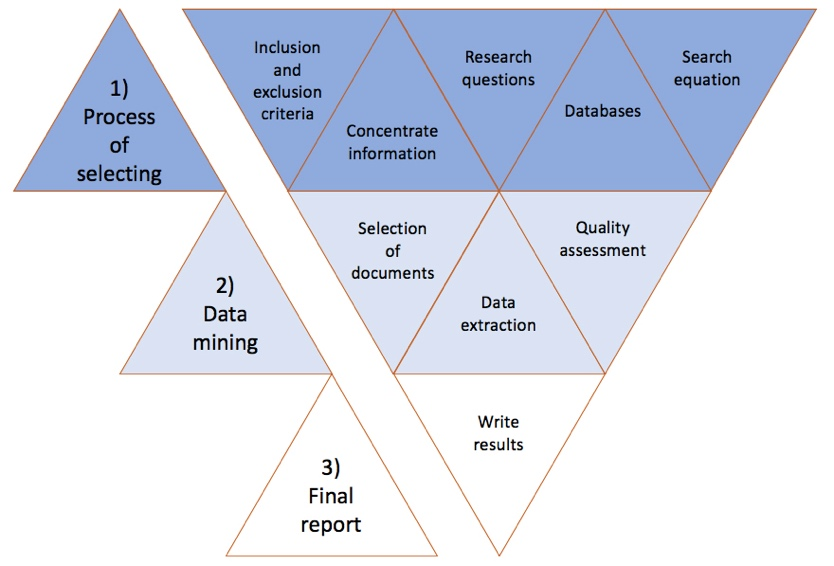
\includegraphics[width=0.6\textwidth]{fig1-33750.jpg}
 \caption{Phases of the present investigation.}
 \label{fig1}
 \source{Own elaboration.}
\end{figure}

\subsection*{Phase 1. Process of selecting}
The Selection Process phase included: determining the research questions, choosing the search equation (\Cref{tab1}), identifying the relevance of the results, discarding the results without open access, eliminating duplicates, assessing the quality of the documents and applying the inclusion criteria (\Cref{fig2}). In the Data Extraction phase, we proceeded to: create the database, fill in the general data fields, answer the research questions and connect the categories supported by keywords. Finally, in the Final Report phase, the organization of the general results, the organization of the information in the database and the analysis to answer the following questions were carried out:

\begin{table}[htpb]
\caption{Systematic Literature Review Process.}
\label{tab1}
\centering
\begin{tabular}{p{0.8cm}p{0.8cm}p{0.8cm}p{0.8cm}|p{0.8cm}p{0.8cm}|p{0.8cm}p{0.8cm}p{1.1cm}|p{0.6cm}p{0.6cm}p{0.6cm}}
\toprule 
\multicolumn{12}{c}{Table 1. Results of the three searches}\\ 
\midrule
& \multicolumn{3}{c}{First search} & \multicolumn{2}{c}{Second search} & \multicolumn{3}{c}{Third search} &
 &
 &
\\ 
\midrule
\rotatebox{90}{\parbox{6cm}{Keywords}} & 
\rotatebox{90}{\parbox{6cm}{Citizen Labs}} & 
\rotatebox{90}{\parbox{6cm}{Innovation Labs; Living Labs}} & 
\rotatebox{90}{\parbox{6cm}{Open City Labs; Social Labs}} & 
\rotatebox{90}{\parbox{6cm}{Social Construction Knowlegde, Open Innovation Labs, Citizen Labs, Innovation Labs, Living Labs, Social Innovation Labs}} &
\rotatebox{90}{\parbox{6cm}{Citizen Labs, Innovation Labs, Living Labs, Social Innovation Labs}} &
\rotatebox{90}{\parbox{6cm}{Citizen Labs, Innovation Labs, Living Labs, Social Innovation Labs}} & 
\rotatebox{90}{\parbox{6cm}{Social Construction Knowlegde, Open Innovation, Citizen Labs, Innovation Labs, Living Labs, Social Innovation Labs}} & 
\rotatebox{90}{\parbox{6cm}{Knowlegde, Open Innovation, Citizen Labs, Innovation Labs, Living Labs, Social Innovation Labs}} &
\rotatebox{90}{\parbox{6cm}{Duplicates eliminated}} &
\rotatebox{90}{\parbox{6cm}{Identify relevance in title and abstract}} &
\rotatebox{90}{\parbox{6cm}{Revised database}}
\\
Scopus & 0 & 0 & 0 & 0 & 0 & 2 & 74 & 4 & & 104 &
\\
WoS & 4 & 16 & 30 & 0 & 0 & 5 & 200 & 0 & & \multirow{3}{=}{\rotatebox{90}{\parbox{2cm}{Evaluate document quality}}} & 
\\
Google scholar & 0 & 0 & 0 & 4 & 3 & 166 & 5 & 0 & & & \\
Sub-totals & 4 & 16 & 30 & 4 & 3 & 173 & 279 & 4 & & & \\
\midrule
Total & \multicolumn{8}{c}{513} & 141 & 95 & 173 \\ 
\bottomrule
\end{tabular}
\source{Own elaboration from the general concentrate.}
\end{table}

\begin{itemize}
\item[RQ 1.] What is the geographical distribution of scientific production related to the Social Construction of Knowledge?
\item[RQ 2.] Which are the journals with the greatest number of publications related to the Social Construction of Knowledge?
\item[RQ 3.] What are the concepts similar to innovation laboratories?
\item[RQ 4.] What are the factors of the Social Construction of Knowledge?
\item[RQ 5.] What are the main findings of the studies analysed?
\item[RQ 6.] What are the challenges found in the publications consulted?
\end{itemize}

\subsection*{Phase 2. Data mining}
The phases of the SLR are described below, with the steps that were followed in each of them. In the first part: selection process, the constructs subject to analysis were determined: SIL, CSK and OI. An initial scan was carried out to specify the search, in order to answer the research questions. In \Cref{tab1}, the search equations are observed. Three moments were carried out to cover the synonyms and translations of the words that guided the search. The inclusion criteria were: 1) Documents published between 2010-2020; 2) Type of document: article or PhD thesis and open access journals. 3) Language of the products: English and Spanish 4) Databases: Scopus (BD-S), Web of Science (BD-W) and Google scholar (BD-G) With the articles that resulted from the searches, the relevance of each document was identified based on the review of the title and the abstract, in addition, those without free access were discarded and, the elimination of duplicates was carried out.

\begin{figure}[htbp]
 \centering
 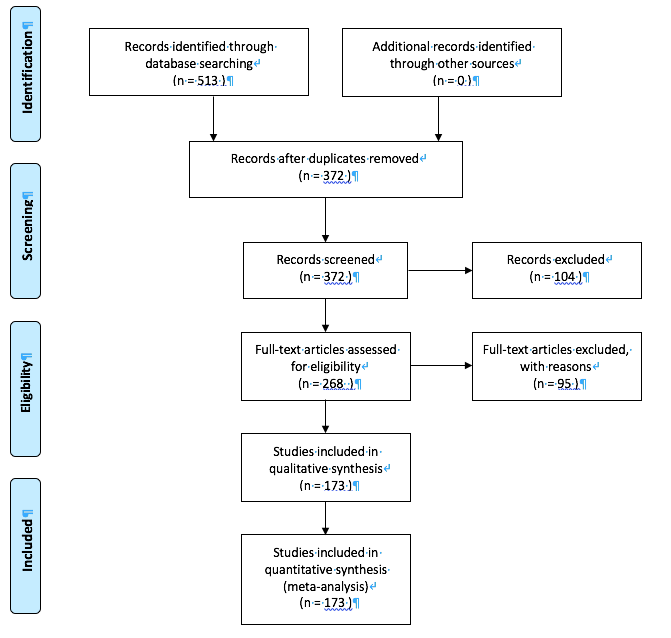
\includegraphics[width=0.75\textwidth]{fig2-33750.png}
 \caption{PRISMA 2009 Flow Diagram.}
 \label{fig2}
 \source{Own elaboration from the general concentrate.}
\end{figure}

As shown in \Cref{fig2}, the total number of documents found was 513, of which 141 duplicates were eliminated. With the identification of relevance of the documents and other 104 were discarded, since the studies were related to the areas of construction, economy, tourism, adult diseases, pharmaceutical field or topics of industrial processes (\Cref{tab1}). The quality of each article was also evaluated and 95 articles that did not show the background of the research or the theoretical framework on the concepts were eliminated: SCK, Laboratories and OI.

\subsection*{Phase 3. Write results}

\section{Results}
\textbf{RQ 1. What is the geographical distribution of scientific production related to the Social Construction of Knowledge?} In \Cref{fig3}, you can see the distribution map of the countries where the items have been produced. Those with more than 10 publications are: Sweden, Germany, Italy, Finland, the Netherlands and Spain, represent 49\% of the total, which are related to Sustainable Development Goal No. 11: Sustainable Cities and Communities.

\begin{figure}[htbp]
 \centering
 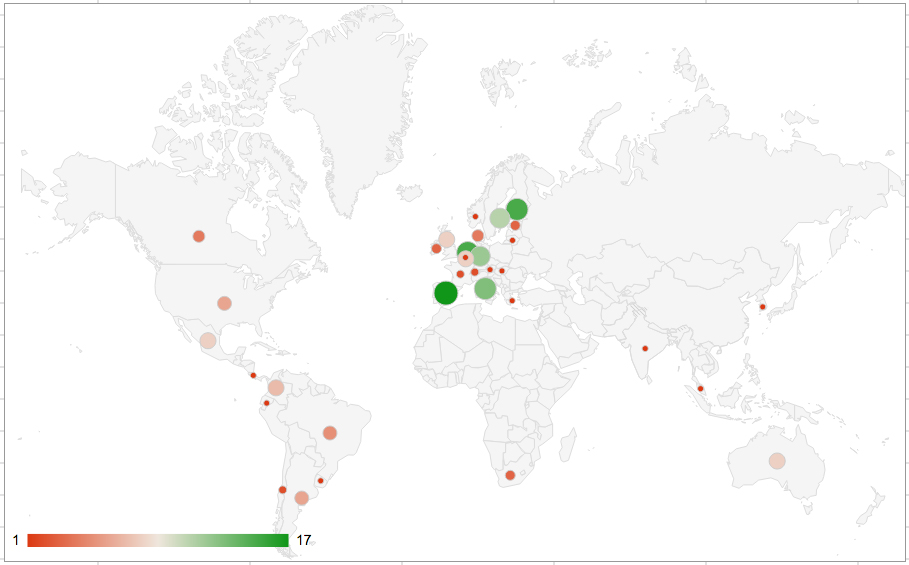
\includegraphics[width=0.7\textwidth]{fig3-33750.jpg}
 \caption{Map of the countries with SIL publications for the Social Construction of Knowledge (SCK).}
 \label{fig3}
 \source{Own elaboration.}
 \notes{The colors order the number of publications in each country in ascending order, starting with red with one publication, to green with 17 publications.}
\end{figure}

\textbf{RQ 2. Which are the journals with the greatest number of publications related to the Social Construction of Knowledge?} \Cref{tab2} shows that at least 8 journals that have published articles on the topic of CSK contain research related to environmental problems and solutions for sustainability. Also, the 10 journals with the highest number of published articles on the topic of CSK through AI-focused laboratories are shown (\Cref{tab2}). Likewise, it is pointed out that the dissemination of knowledge is published in high impact Scopus journals (Q1 and Q2), even though two of the journals with more publications are indexed in Google Scholar.

\begin{table}[htpb]
\caption{Systematic Literature Review Process.}
\label{tab2}
\centering
\begin{tabular}{p{0.3\textwidth}p{0.16\textwidth}p{0.08\textwidth}p{0.08\textwidth}p{0.23\textwidth}}
\toprule 
Journal & Database & Quartile & Number of articles & Article number identification
\\
\midrule
Technology Innovation Management Review & Google scholar & No & 13 & 10, 14, 19, 20, 31, 32, 33, 38, 44, 46, 53, 58, 66
\\
*Sustainability & Scopus & Q2 & 6 & 105, 107, 108, 112, 114, 155
\\
*Revista Iberoamericana de Ciencia, Tecnología y Sociedad & Google scholar & No & 9 & 1, 26, 62, 63, 64, 73, 83, 95, 96
\\
*GAIA-Ecological Perspectives for Science and Society & Scopus & Q2 & 4 & 22, 56, 121, 123
\\
*Energy Research \& Social Science & Scopus & Q1 & 3 & 28, 119, 142
\\
*Journal of Cleaner Production & Scopus & Q1 & 3 & 3, 102, 154
\\
Journal of Service Theory and Practice & Scopus & Q1 & 2 & 50, 59
\\
*Renewable Energy & Scopus & Q1 & 2 & 9, 136
\\
Telematics and Informatics & Scopus & Q1 & 2 & 40, 52
\\
*International Journal of Sustainability in Higher Education & Scopus & Q2 & 2 & 133, 161
\\
Technology Analysis \& Strategic Management & Scopus & Q2 & 2 & 4, 54
\\ 
\bottomrule
\end{tabular}
\source{Own elaboration.}
\end{table}

\textbf{RQ 3. What are the concepts similar to innovation laboratories?} A classification of the number of articles per type of laboratory was made and a cross with the SDG [Sustainable Development Goals] (\Cref{tab3}). Most of the articles (131) refer to living laboratories and relate them to: Industry, innovation and infrastructure (52); Sustainable cities and communities (49). It should be noted that in most of the laboratories the central SDG are Sustainable cities and communities (68) and Industry innovation and infrastructure (64). Based on this information, an area of opportunity to respond to environmental problems through the creation of laboratories related to: Responsible production and consumption, and Climate action.

\begin{table}[htpb]
\caption{Similar concepts from the Labs and the relationship with SDG.}
\label{tab3}
\centering
\begin{tabular}{p{0.24\textwidth}|p{0.04\textwidth}p{0.04\textwidth}p{0.04\textwidth}p{0.04\textwidth}p{0.04\textwidth}p{0.04\textwidth}p{0.04\textwidth}p{0.04\textwidth}p{0.04\textwidth}p{0.04\textwidth}|p{0.04\textwidth}}
% \toprule 
\multicolumn{1}{c}{} & \multicolumn{1}{c}{\rotatebox{90}{\parbox{6cm}{Climate action}} }
& \rotatebox{90}{\parbox{6cm}{Decent work and economic growth}} 
& \rotatebox{90}{\parbox{6cm}{Gender Equality}} 
& \rotatebox{90}{\parbox{6cm}{Health and wellness}} 
& \rotatebox{90}{\parbox{6cm}{Industry, innovation and infrastructure}} 
& \rotatebox{90}{\parbox{6cm}{Partnerships to achieve the objectives}} 
& \rotatebox{90}{\parbox{6cm}{Quality education}} 
& \rotatebox{90}{\parbox{6cm}{Reducing inequalities}} 
& \rotatebox{90}{\parbox{6cm}{Responsible production and consumption}} 
& \rotatebox{90}{\parbox{6cm}{Sustainable cities and communities}} 
& \rotatebox{90}{\parbox{6cm}{Total number of articles}}
\\
\midrule
Citizen labs & & & & & 1 & & & & & 6 & 7
\\
Innovation labs & 1 & & & 1 & 10 & & 4 & 1 & 1 & 11 & 29
\\
Living labs & 1 & 2 & & 8 & 52 & 1 & 13 & 1 & 4 & 49 & 131
\\
Social Innovation labs & & & & & & 1 & 1 & & & 2 & 4
\\
Virtual labs & & & 1 & & 1 & & & & & & 2
\\
Sub-total & 2 & 2 & 1 & 9 & 64 & 2 & 18 & 2 & 5 & 68 &
\\
\midrule
Total & \multicolumn{11}{c}{173}
\\ 
\bottomrule
\end{tabular}
\source{Own elaboration.}
\end{table}

\textbf{RQ 4. What are the factors of the Social Construction of Knowledge?} The data from RQ 4 was cross-checked with the areas of the society to determine where the SCK is being promoted. The factors of SCK are knowledge creation, use of technology, communicative interaction, disciplinary fields, and dissemination of knowledge. In 52 articles it was found that the participation of different disciplinary fields is a factor for KCS and one of the disciplinary fields is Education as the predominant area with 65 investigations, followed by Environment (29), Culture (20), Politics (18), Science (17), Economy (15) and Health with 9 (\Cref{fig4}). Education is the area where the interest in laboratories prevails, as a way to respond to the SCK, which represents valuable information for the universities that gather the actors of the quadruple helix to consolidate learning, teaching and research spaces, addressing diverse topics, such as: Sustainable cities and communities, industry, innovation and infrastructure.

\begin{figure}[htbp]
 \centering
 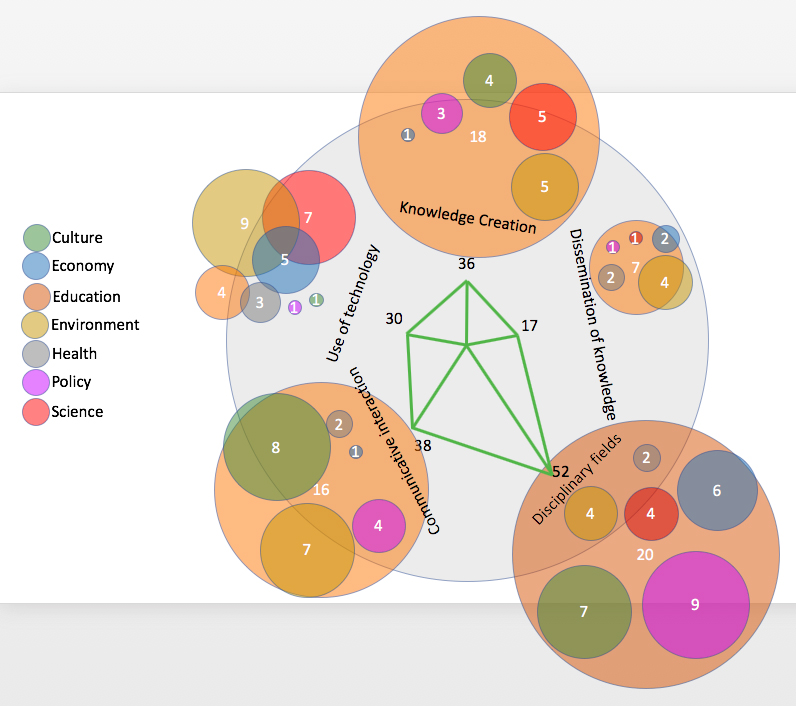
\includegraphics[width=0.7\textwidth]{fig4-33750.jpg}
 \caption{Characteristics of the Social Construction of Knowledge (SCK).}
 \label{fig4}
 \source{Own elaboration.}
\end{figure}

\textbf{RQ 5. What are the main findings of the studies analyzed?} In the SLR, 72 articles were found that mention that collaborative spaces, such as SIL, are driven by the motivation to create prototypes to generate scalable solutions and offer evidence that the different actors of the quadruple helix have been connected for this purpose (\Cref{fig5}). In addition, 32 articles show that training in non-formal settings allows for the creation of open science and different forms of development of societies, which leads to the issue of free access to knowledge. The OI refers to Open Science, 25 articles were located related to the topic and the contribution to society seeking the common good through open knowledge is highlighted, which is closely related to the concept of OI. On the other hand, in 19 articles, the importance of the friendliness with the environment is exposed and they confirm the attention of topics on the care of the environment through collective commitments with practices based on the technique of learning by doing and in 16 articles the need of the continuous education is exposed that allude to the topics: closing of the digital gap, access to the information, education with the format of experimentation for the creation of prototypes and social reality.

\begin{figure}[htbp]
 \centering
 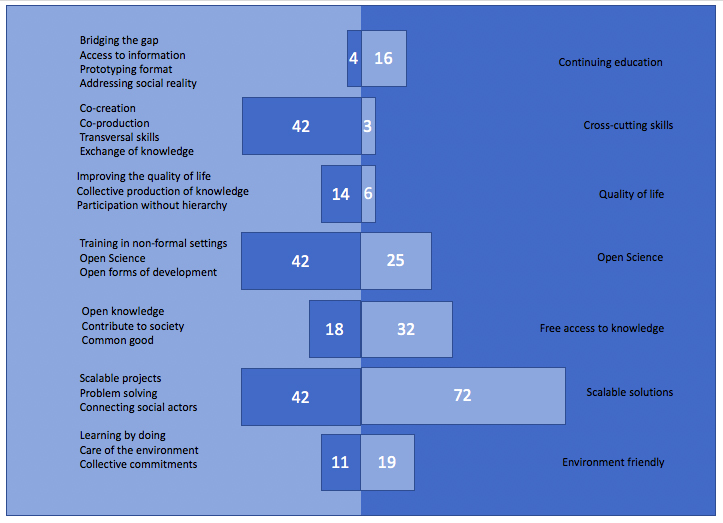
\includegraphics[width=0.7\textwidth]{fig5-33750.jpg}
 \caption{Categories of Open Innovation.}
 \label{fig5}
 \source{Adapted categories (left) \cite{yanez-figueroa2016} and Open Innovation (right) \cite{dellera2014}.}
\end{figure}

\textbf{RQ 6. What are the challenges found in the publications consulted?} \Cref{fig6} shows that 72 articles set out the challenge of development towards the knowledge and information society; 26 set out the need to increase literacy and environmental awareness. Likewise, the remaining 22 articles mention the need to boost through OI the decentralized production systems in order to be more competitive, which will allow the transformation of the value and lifestyle of society in general.

\begin{figure}[htbp]
 \centering
 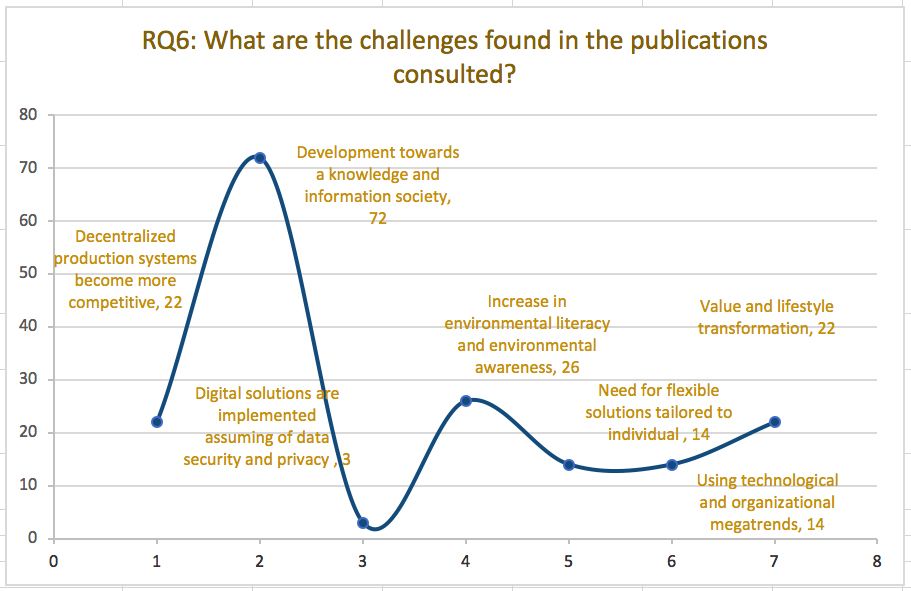
\includegraphics[width=0.7\textwidth]{fig6-33750.jpg}
 \caption{Challenges of the Social Construction of Knowledge (SCK).}
 \label{fig6}
 \source{Own elaboration.}
 \notes{On the Y-axis, the number of articles is shown, and on the X-axis, the categories by \textcite{walz2019}.}
\end{figure}

\section{Discussion}
The SIL have also been called living laboratories or innovation laboratories, in their different formats they open a range of possibilities to create knowledge from the OI approach as a common science for the care of the environment. In the SLR, 131 articles were found that refer to living laboratories and 29 to innovation laboratories (\Cref{tab3}). According to \textcite{castro2020, zambrano2020}, the environment is one of the central themes of the Stockholm Declaration (1972), the World Charter for Nature (1982), the Rio Declaration on Environment and Development (1992) and the United Nations Conference on Sustainable Development (2012), which contemplate various regulations, principles and strategies to be followed for its protection. The SLR carried out in the period of the last 10 years, confirms that the efforts of the different sectors of the society (quadruple helix: citizen, company, government and school) take care of subjects of the area of the natural sciences, but greater shared efforts are required -in SIL- for the creation of public policies, laws, regulations and national and international agreements for the care, conservation and protection of the environment.

SIL participants come from different disciplinary fields which is one of the relevant factors for SCK and the educational field is one of the most sensitive for producing knowledge from these experimental approaches. The study found that 52 articles talk about the involvement of different disciplinary fields as a factor for SCK and that the disciplinary field of Education is the predominant area with 65 investigations (\Cref{fig4}). This is a novel option that is still growing, since the exchange of knowledge and experiences in everyday life and political positions needs to be consolidated in order to cement successful projects by providing continuity and seeking permeability in similar contexts around the world \cite{garcia+lopez2020}. In the same vein, \textcite{evans2015} and \textcite{alonso2020} reaffirm that schools are using the Innovation Lab model as a disruptive proposal for the SCK and as emerging spaces for action-research.  In short, for the SSC to be carried out in the SIL, with an open science approach, it is necessary to consider bringing together different disciplinary fields to build and disseminate knowledge using ICT with face-to-face communicative interaction models.

The SIL are governed by the motivation of creating prototypes to generate solutions, in addition, they have allowed experimentation in real contexts, to address global problems, such as environmental conservation. This is strengthened by the entrepreneurial, research and educational activities carried out in Fab Labs as their solutions can then be shared with similar communities around the world and multiplied by collaboration with shared innovation \cite{wolf-powers2017}. In the RSL 72 articles mention that the collaborative spaces to generate scalable solutions giving play to the participation of the different agents of the quadruple helix are the Laboratories (\Cref{fig5}). This coincides with the studies by \textcite{baran2020} and \textcite{barbancho2020}, who state that AI remains an emerging approach due to the validation of results by users, who are responsible for testing products, services or processes when they are part of the experimental environments of the Laboratories. Thus, these are consolidated with the application in different contexts and are enriched with the participation of people coming from diverse areas of knowledge. 

The SLR has been a tool to corroborate that sustainability has challenges to shape interdisciplinary projects to address problems with climate, responsible production and consumption, while confirming challenges in the actions for the development of the knowledge society. In this study 72 articles are presented with the challenge of development towards the knowledge and information society; and, 26 with the theme of literacy and environmental awareness (\Cref{fig6}). The previous findings allow for awareness of the importance of contributing in a transversal manner to the needs of society and to the pending efforts to generate environmental policies, laws, regulations and international agreements aimed at caring for and protecting the environment \cite{estevez-alvarez2020}. It should also be pointed out that the complexity of environmental issues requires the participation of interdisciplinary groups to collaborate from the different fields of science, in order to prototype solutions to the problems posed and, subsequently, to corroborate their application and implementation in the knowledge society \cite{peduzzi2020}. From this perspective, commitments can be made to increase responses to demands related to the environment, people in vulnerable situations, science and technology \cite{mikhak2002}, in such a way that options are opened up to continue building and socializing knowledge towards a sensitive and responsible society.

\section{Conclusion}
Laboratories, in their different modalities, are a training option, since they are viable for attending UNESCO's SDG through interdisciplinary groups that promote SCK through the participation of different actors in society. In that sense, considering the makerspace movement as part of the sector of the population -citizens- who freely share the specifications of their prototypes for others to reproduce. The quadruple helix is involved in the work with SIL, however, the necessary planning was manifested with the intervention of the area of education, which was the main driver of the research reported in this SLR, which was reflected in the integration of universities, schools, research centers and teaching groups. Therefore, it was identified that universities are the source of knowledge production that most promotes these spaces, and that they assume the commitment of disseminating project results in their institutional repositories. 

SIL are positioned as decentralized knowledge production systems and the results they generate are competitive due to the OI approach. It is relevant to consider that the topics related to the environment are the most attended in the SIL, for that reason the urgent necessity to continue mobilizing knowledge through these spaces where flexible solutions are produced and adapted to the individuals, with the support of specialists of the different areas from the science. Consequently, great efforts are being made to focus research on issues such as: quality of life, open science and open access, which are key to the development of society. The Laboratories are based on the aspects mentioned above, since they offer the possibility of creating spaces for experimentation in benefit of sustainability, used as a transversal theme. Some of the pending challenges to be addressed in the SIL are literacy and environmental awareness, since interdisciplinary experiences are promoted in these spaces. In order to contribute to these studies, the SLR allows mapping the areas where formal research has been carried out and evidences the challenges that still need to be faced in order to consolidate the SIL and the SCK from the OI approach. 

\printbibliography\label{sec-bib}
% if the text is not in Portuguese, it might be necessary to use the code below instead to print the correct ABNT abbreviations [s.n.], [s.l.] 
%\begin{portuguese}
%\printbibliography[title={Bibliography}]
%\end{portuguese}

%full list: conceptualization,datacuration,formalanalysis,funding,investigation,methodology,projadm,resources,software,supervision,validation,visualization,writing,review
\begin{contributors}[sec-contributors]
\authorcontribution{José-Antonio Yañez-Figueroa}[conceptualization,formalanalysis,investigation,projadm,visualization,writing,review]
\authorcontribution{María-Soledad Ramírez-Montoya}[funding,formalanalysis,methodology,review,conceptualization,supervision]
\authorcontribution{Francisco-José García-Peñalvo}[funding,formalanalysis,methodology,review,conceptualization,supervision]
\end{contributors}


\end{document}
